\documentclass{beamer}
\usepackage{amsmath}
\usepackage{enumitem}
\usepackage{graphicx}
\usepackage{pdflscape}
\usepackage{float}

\begin{document}

\title{CS572 - Lecture note}
\subtitle{Group 12, The Kip-reader's}
\author{Houjeung Han \and Jesper Loenbaek \and Youngsoo Jang}
\institute%
{
    School of Computing\\
    KAIST\\
    Daejeon, Korea
}

\date{16 Nov 2016}
\frame{\titlepage}

\begin{frame}{Controller Stability}
    \begin{columns}[T]
    \column{.5\textwidth}
    \begin{align*}
        \dot{x} =& f(\bar{x},\bar{y},\bar{t})\\
        \dot{u} =& y(\bar{x},\dot{t})\\
        \dot{\bar{x}} =& f(\bar{x}^*,t)
    \end{align*}
    *equality point
    \column{.5\textwidth}
    \end{columns}
\end{frame}

\begin{frame}{pendulum}
    \begin{columns}[T]
    \column{.6\textwidth}
    System Equation
    $$MR^2 \ddot{\theta} + b\dot{\theta} + MgRsin(\theta)=0$$
    %
    let
    \vspace*{-0.5cm}
    \begin{align*}
        x_1 =& \theta\\
        x_2 =& \dot{\theta}
    \end{align*}
    \vspace*{-1cm}
    \begin{align*}
        \dot{x}_1 =& x_2\\
        \dot{x}_2 =& \frac{-b}{MR^2}x_2-\frac{g}{R}sin(x_1)=0
        %\dot{x}_2 =& \frac{-b}{MR^2}x_2-\frac{g}{R}sin(\theta)=0
    \end{align*}
    Eq point $\Rightarrow \; x_2=0,\; sin(x_1)=0,\; \theta=0,\pi$
    \column{.4\textwidth}
        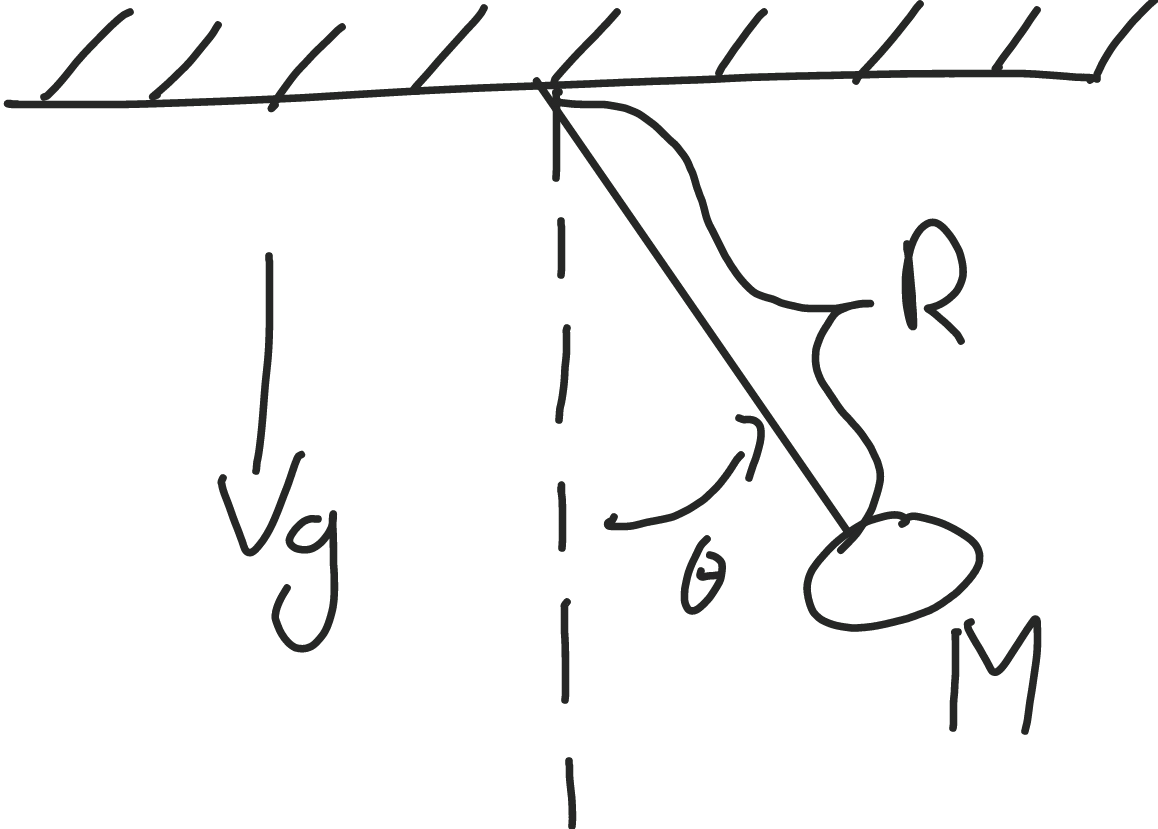
\includegraphics[width=\textwidth]{fig/pendulum.png}   
    \end{columns}
\end{frame}

\begin{frame}{pendulum (1)}
    \begin{columns}[T]
    \column{.6\textwidth}
    Van der Pol Oscilator
    \begin{align*}
        \dot{x}_1 =& x_2\\
        \dot{x}_2 =& -x_2+(1-x^2)-x_2
    \end{align*}
    %
    \vspace{1cm}
    $$\forall R\supset 0,\; \exists r>0,\; ||x(0)||<\gamma \Rightarrow \forall t>0,\;||x(t)||<R$$
    \column{.4\textwidth}
        \vspace{-1cm}
        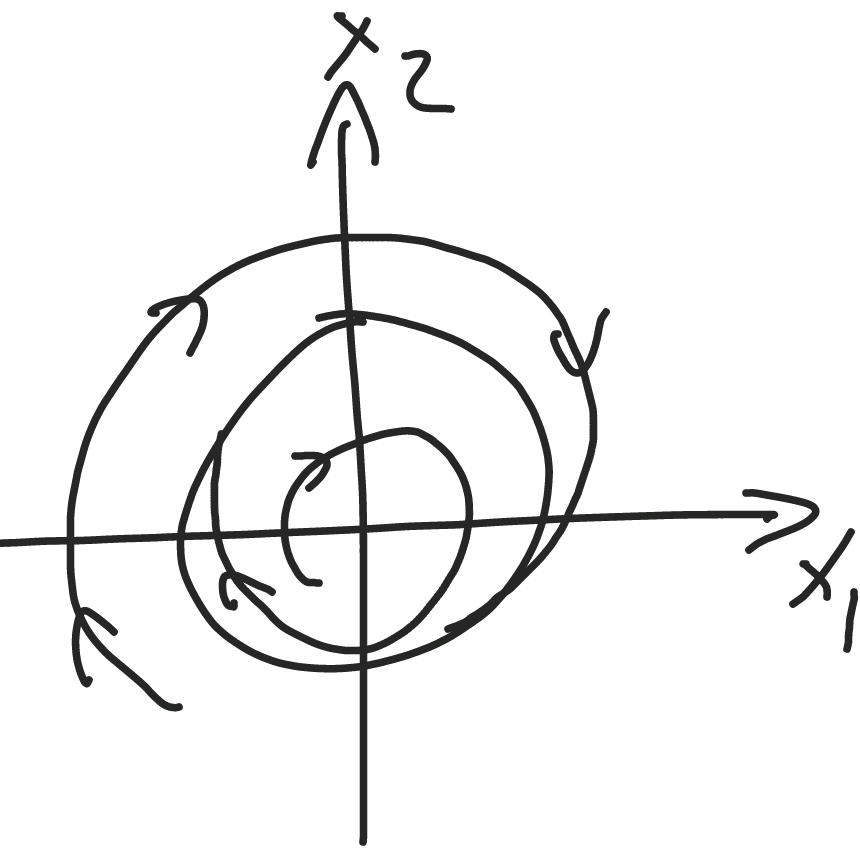
\includegraphics[width=\textwidth]{fig/limitCircle.png}   
    \end{columns}
\end{frame}

\begin{frame}{pendulum (2)}
    \begin{columns}[T]
    \column{.6\textwidth}
    Lyapunov Stability\\
    $$\Rightarrow x(t)\rightarrow 0 \; as\; t\rightarrow \infty$$
    \hspace{1cm}(1) Marginally stable\\
    \hspace{1cm}(2) Asymptotically stable\\
    \hspace{1cm}(3) Unstable\\
    \hspace{1cm}(*) Exponentially stability\\
    \column{.4\textwidth}
        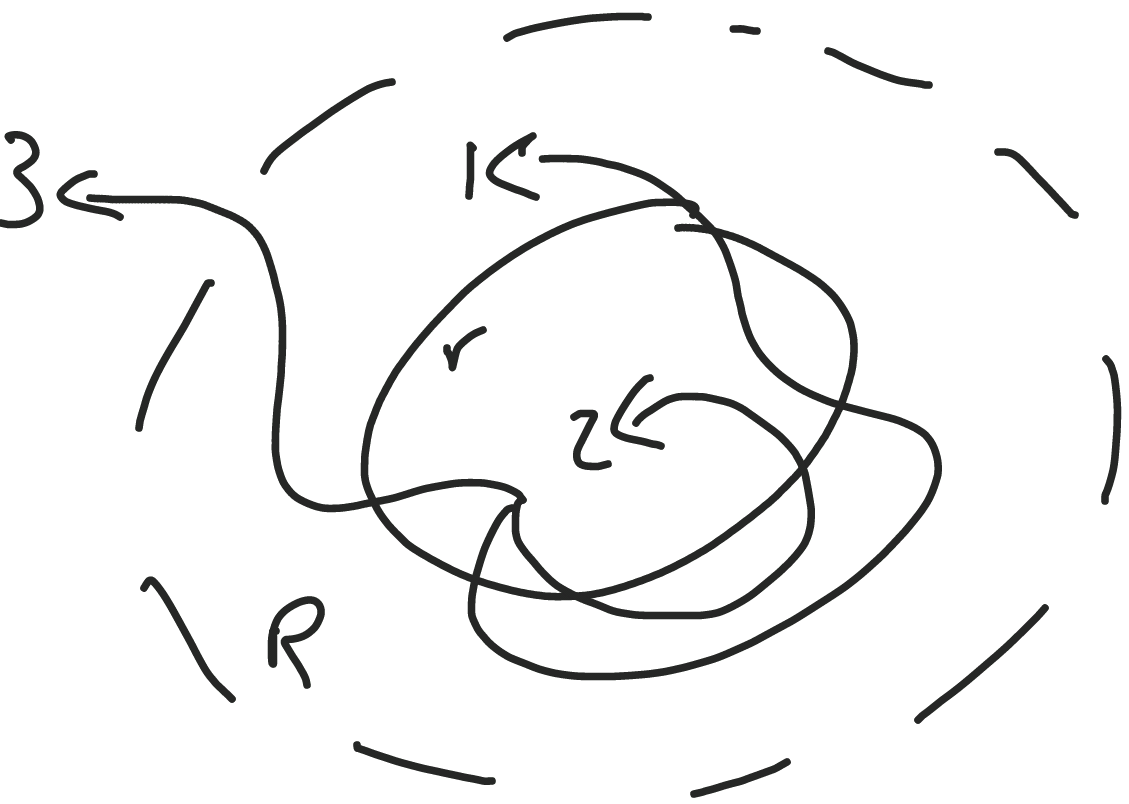
\includegraphics[width=\textwidth]{fig/lyapunovStability.png}   
    \end{columns}
\end{frame}

\begin{frame}{$V(x)$ Scalar, smooth}
$$\dot{v} = \frac{d}{dt}v(\bar{x}),\; v^T = f(x)$$
$$v(\bar{x})\rightarrow {\infty}^+ \; as\; ||\bar{x}|| \rightarrow {\infty}^+$$
$$\& \dot{v}(\bar{x}) \leq 0 \; for \; \forall \bar(x)$$
Let $R$ be the set where $\dot{x}=x$ then any of the system tends towards the largest invariant set within $R$ 
\end{frame}

\begin{frame}{Invariant Set}
Starts there, stay there\\
Let
$$v=\frac{1}{2}\dot{x}^2+\int_0^x C(x)dx$$
\vspace{-1cm}
\begin{align*}
    &|x| \rightarrow \infty \Rightarrow \infty\\
    &|x| \rightarrow \infty \Rightarrow \infty\\
\end{align*}

\begin{align*}
    &xC(x)>0\; for\; x \neq 0\\
    &\dot{x}b(\dot{x}) > 0\; for\; \dot{x} \neq 0
\end{align*}
\end{frame}

%Invariant set
\begin{frame}{ex}
    \begin{columns}[T]
    \column{.5\textwidth}
        $\ddot{x}+b(\dot{x})+C(x)=0$\\
        \vspace{1cm}
        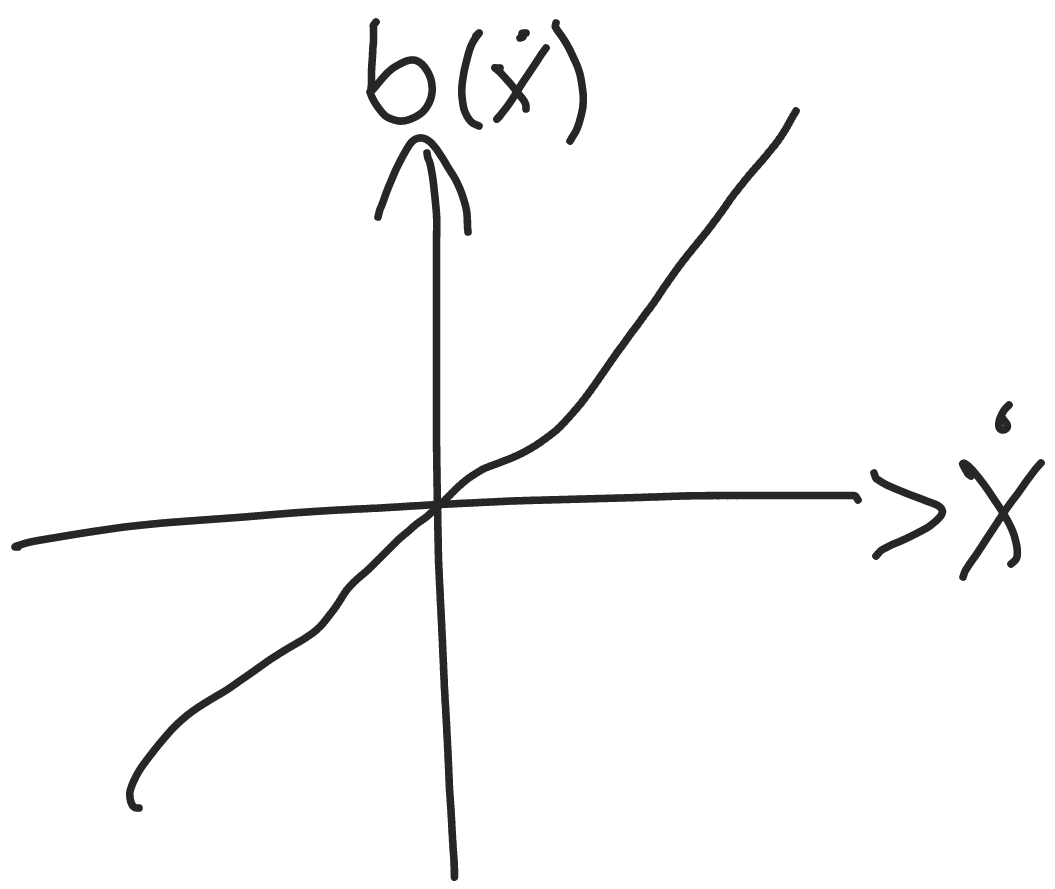
\includegraphics[width=\textwidth]{fig/bx.png}   
    \column{.5\textwidth}
        \vspace{1cm}
        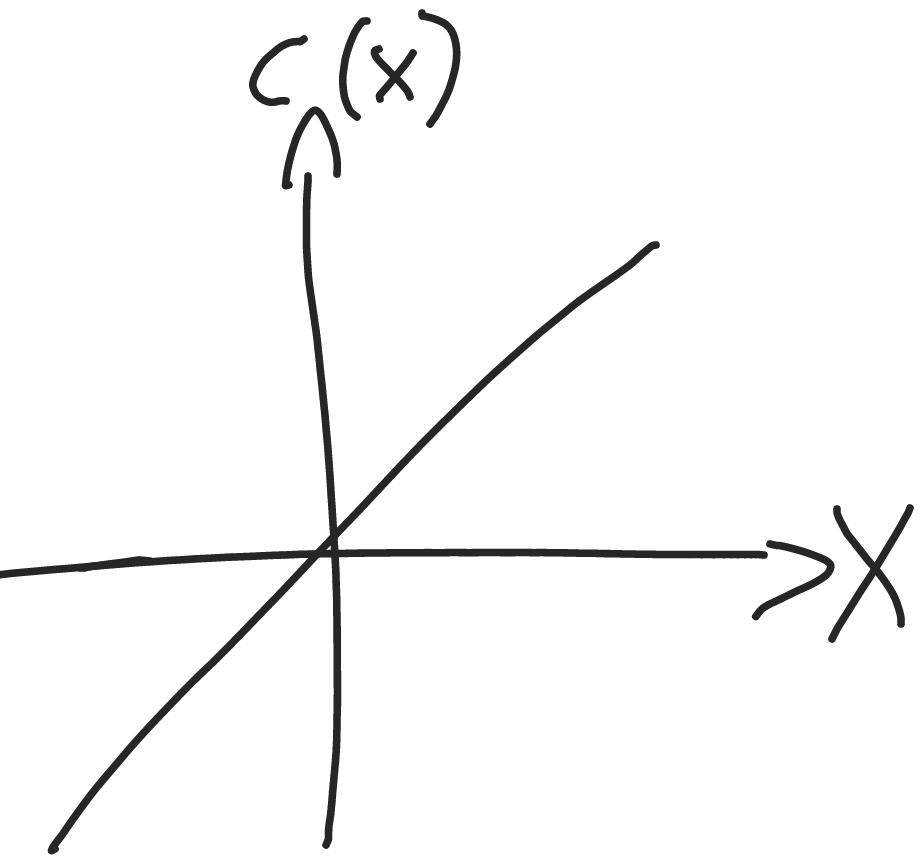
\includegraphics[width=0.9\textwidth]{fig/cx.png}   
    \end{columns}
\end{frame}

\begin{frame}{ex (2)}
    $\dot{v}=\dot{x}\ddot{x} + \frac{d}{dt}f^x_0 C(x)dx \dot{x} = \dot{x}(-b(\dot{x}))=\dot{x}b(\dot{x})<0$\\
    $v=0 \Rightarrow \dot{x}=0$\\
    $\bar{\ddot{x}}-C(x) \neq 0\; unless\; 0$\\
\end{frame}

\begin{frame}{Real Robot}
    \begin{align*}
        &H(\dot{b})\ddot{\bar{b}}+ C(\bar{q},\ddot{\bar{q}})\bar{q}+g(\bar{q})=\tau\\
        &\bar{\tau}=g(\bar{q})-(K_p-q+k_D\dot{\bar{g}}), \; \tilde{\bar{q}}=\bar{q}-\bar{q}_d\\
        &V=\frac{1}{2}\dot{q}^\tau H \dot{g}+ \frac{1}{2} \tilde{q}^\tau K_p \tilde{q}
    \end{align*}
    \begin{align*}
    \frac{d}{dt}(\frac{1}{2} q^\tau H \dot{q}) =& \frac{1}{2} \bar{q} \dot{H}\dot{g}+\frac{1}{2}q^\tau +Hg\\
    =& \bar{q}^+ H\bar{g}+\frac{1}{2}\dot{q}^\tau \dot{H}\dot{q}\\
    =& \bar{q}^+ (\bar{\tau}-\bar{q}-C\bar{q})+\frac{1}{2}\bar{g}H\bar{q}\\
    =& q^\tau(\bar{\tau}-q)
    \end{align*}
\end{frame}

\begin{frame}{Real Robot(2)}
    \begin{align*}
        \frac{d}{dt} (\frac{1}{2}g^\tau H\dot{g})+&\int_0^t g^\tau d\bar{g} = \bar{g}^\tau \tau\\
        &\int_0^t g^\tau g dt
    \end{align*}
    $$\dot{q}^\tau(H-2C)\bar{q}=0\forall \dot{\bar{q}}$$

    $x^\tau Mx = 0$ (skew symmetric)\\
    $M=-m^\tau$
\end{frame}

\begin{frame}{Real Robot(3)}
    \begin{align*}
        \dot{v} =& \dot{\bar{q}}^\tau (\bar{\tau}-\bar{g})+\bar{q}^\tau k_p \bar{q}\\
        =& \dot{\bar{q}}^\tau(q-k_p \bar{q}-k_0 \bar{q}-\bar{q}k_p \tilde{q})\\
        =& -\dot{\bar{q}}^\tau k_p \bar{q} \leq 0
    \end{align*}
    $$\dot{\bar{g}}=0$$
    $$H\ddot{g}=\tau-q=-K_q=-K_p\bar{q}=0, \; \tilde{q}=0$$
\end{frame}

\end{document}
